% 

\documentclass[aspectratio=169]{beamer}

\usetheme{Madrid}
\usecolortheme{seahorse}

\usepackage[version=4]{mhchem}
\usepackage{chemfig}
\usepackage{amsmath}
\usepackage{siunitx}
\usepackage{tikz}
\usetikzlibrary{arrows.meta,calc,positioning,decorations.pathmorphing,shapes.geometric}

\title[Fuel Naming]{Organic Chemistry Naming for Combustion\\ with Fuels Emphasis}
\author{Prof. Dr. Onur Tuncer}
\institute{Aeronautical Engineering \\ Istanbul Technical University}
\date{}

% ---------- Simple "3D-ish" ball-and-stick TikZ helpers ----------
\newcommand{\atom}[4]{% name, x,y, label
  \node[circle, draw, fill=white, minimum size=9mm, inner sep=0pt] (#1) at (#2,#3) {\small #4};
}
\newcommand{\bondback}[2]{\draw[black!35, line width=1.2pt] (#1) -- (#2);}
\newcommand{\bondfront}[2]{\draw[black, line width=1.6pt] (#1) -- (#2);}

% ---------- Flame drawing helper (grayscale + opacity) ----------
\newcommand{\flameicon}[1]{%
\begin{tikzpicture}[scale=#1]
  \draw[rounded corners=2pt, fill=black!10] (-0.4,-0.6) rectangle (0.4,-0.2);
  \draw[fill=black!15] (-0.25,-0.2) rectangle (0.25,0.0);
  \draw[decorate, decoration={random steps, segment length=2.5pt, amplitude=1.3pt},
        fill=black!8, draw=black!30] (0,0) .. controls (-0.55,0.55) and (-0.35,1.15) .. (0,1.55)
                                      .. controls (0.35,1.15) and (0.55,0.55) .. (0,0) -- cycle;
  \draw[decorate, decoration={random steps, segment length=2.2pt, amplitude=1.0pt},
        fill=black!18, draw=black!45] (0,0.05) .. controls (-0.38,0.45) and (-0.22,0.95) .. (0,1.20)
                                      .. controls (0.22,0.95) and (0.38,0.45) .. (0,0.05) -- cycle;
\end{tikzpicture}%
}

% ---------- A "naming recipe" macro for consistent slides ----------
\newcommand{\namingrecipe}{
\begin{block}{Naming recipe (do this every time)}
\begin{enumerate}
\item Find parent: \textbf{longest chain} (or ring) containing key functional group / multiple bond
\item Pick suffix: \textbf{-ane, -ene, -yne} or functional-group suffix
\item Number parent to give \textbf{lowest locants} (priority: multiple bonds, then substituents)
\item Name substituents (methyl, ethyl, propyl, \dots) + positions
\item Alphabetize substituents (ignore di-, tri-, tetra-), assemble full name
\end{enumerate}
\end{block}
}

\begin{document}

%------------------------------------------------
\begin{frame}
\titlepage
\end{frame}

%------------------------------------------------
\begin{frame}{Why naming is a combustion skill?}
\begin{itemize}
\item In combustion papers, you will see species lists, surrogates, mechanisms:
  \(\text{n-dodecane, iso-octane, methyl-cyclohexane, toluene,}\dots\)
\item Naming \(\Rightarrow\) structure recognition \(\Rightarrow\) ignition/soot intuition
\item Aviation fuels are mixtures: naming helps classify components quickly
\end{itemize}
\centering\vspace{2mm}
\flameicon{0.65}\hspace{6mm}\flameicon{0.65}\hspace{6mm}\flameicon{0.65}
\end{frame}

%------------------------------------------------
\begin{frame}{Today’s focus}
\begin{enumerate}
\item Hydrocarbon naming: alkanes, cyclo-alkanes, alkenes, aromatics
\item Substituents + numbering: branching and rings (relevant to fuel)
\item Oxygenates (brief): alcohols, ethers, esters (blending relevance)
\item Quick combustion mapping: octane versus structure, soot tendency, aviation notes
\end{enumerate}
\end{frame}

%------------------------------------------------
\begin{frame}{Minimal dictionary: prefixes (parent chain length)}
\begin{center}
\begin{tabular}{c c c c}
meth- & 1 & hex- & 6 \\
eth- & 2 & hept- & 7 \\
prop- & 3 & oct- & 8 \\
but- & 4 & non- & 9 \\
pent- & 5 & dec- & 10 \\
\end{tabular}
\end{center}

\vspace{2mm}
Fuel context: jet fuels are often \(\mathrm{C_8\!-\!C_{16}}\) families.
\end{frame}

%------------------------------------------------
\begin{frame}{Step 0: draw the carbon skeleton fast}
\begin{columns}[T,onlytextwidth]
\column{0.55\textwidth}
\begin{itemize}
\item Ignore H atoms at first
\item Find the longest continuous carbon path
\item Mark branches as substituents
\end{itemize}

\column{0.45\textwidth}
\centering
\chemfig{H_3C-CH(-CH_3)-CH_2-CH_3}

\vspace{1mm}
Skeletal view: longest chain = 4 (butane), methyl at C-2
\end{columns}
\end{frame}

%------------------------------------------------
\begin{frame}{Core naming recipe}
\namingrecipe
\end{frame}

%------------------------------------------------
\begin{frame}{Alkanes: suffix \textbf{-ane} (fuel backbone)}
\begin{block}{Straight chain example}
\centering
\chemfig{H_3C-CH_2-CH_2-CH_3}

\vspace{1mm}
\textbf{butane}
\end{block}

\begin{itemize}
\item n-alkanes: key in diesel/jet surrogates (e.g., n-dodecane)
\item As chain grows: volatility \(\downarrow\), boiling point \(\uparrow\)
\end{itemize}
\end{frame}

%------------------------------------------------
\begin{frame}{Substituents: alkyl groups}
\begin{center}
\begin{tabular}{c c}
methyl & \(\ce{-CH3}\) \\
ethyl & \(\ce{-CH2CH3}\) \\
propyl & \(\ce{-CH2CH2CH3}\) \\
isopropyl & \(\ce{-CH(CH3)2}\) \\
tert-butyl & \(\ce{-C(CH3)3}\) \\
\end{tabular}
\end{center}

\vspace{2mm}
Fuel context: branching (methyl/ethyl branches) \(\Rightarrow\) octane \(\uparrow\).
\end{frame}

%------------------------------------------------
\begin{frame}{Rule: choose the \textbf{longest chain}}
Name the parent correctly first.

\begin{columns}[T,onlytextwidth]
\column{0.55\textwidth}
\centering
\chemfig{H_3C-CH(-CH_3)-CH_2-CH_2-CH_3}

\vspace{1mm}
Longest chain = 5 \(\Rightarrow\) pentane parent

\column{0.45\textwidth}
\begin{itemize}
\item Parent: pentane
\item Substituent: methyl
\item Position: 2
\end{itemize}
\end{columns}

\begin{block}{Name}
\textbf{2-methylpentane}
\end{block}
\end{frame}

%------------------------------------------------
\begin{frame}{Rule: number to give the \textbf{lowest locants}}
\begin{columns}[T,onlytextwidth]
\column{0.52\textwidth}
\centering
\chemfig{H_3C-CH_2-CH(-CH_3)-CH_2-CH_3}

Option A numbering (left-to-right) gives methyl at 3.

\column{0.48\textwidth}
\centering
\chemfig{H_3C-CH_2-CH_2-CH(-CH_3)-CH_3}

Option B numbering (right-to-left) gives methyl at 2.
\end{columns}

\begin{block}{Correct name}
\textbf{2-methylpentane} (choose lowest number)
\end{block}
\end{frame}

%------------------------------------------------
\begin{frame}{Multiple substituents: di-, tri-, tetra-}
\centering
\chemfig{H_3C-CH(-CH_3)-CH(-CH_3)-CH_3}

\vspace{2mm}
\begin{itemize}
\item Parent: butane
\item Substituents: methyl at 2 and 3
\end{itemize}

\begin{block}{Name}
\textbf{2,3-dimethylbutane}
\end{block}
\end{frame}

%------------------------------------------------
\begin{frame}{Alphabetical order (ignore di-, tri-, tetra-)}
\centering
\chemfig{H_3C-CH(-CH_2CH_3)-CH(-CH_3)-CH_2-CH_3}

\vspace{2mm}
\begin{itemize}
\item Parent: pentane
\item Substituents: ethyl and methyl
\item Numbering: ethyl at 2, methyl at 3 (lowest set)
\end{itemize}

\begin{block}{Name}
\textbf{2-ethyl-3-methylpentane} (E before M)
\end{block}
\end{frame}

%------------------------------------------------
\begin{frame}{Branching intensity and octane (gasoline intuition)}

\begin{columns}[T,onlytextwidth]
\column{0.5\textwidth}
\begin{block}{n-Heptane (PRF 0)}
\centering
\chemfig{H_3C-CH_2-CH_2-CH_2-CH_2-CH_2-CH_3}
\end{block}

\column{0.5\textwidth}
\begin{block}{Iso-octane (PRF 100)}
\centering
\chemfig{H_3C-C(-CH_3)(-CH_3)-CH_2-CH(-CH_3)-CH_3}
\end{block}
\end{columns}

\begin{itemize}
\item More branching \(\Rightarrow\) higher octane (more knock resistance)
\item Naming makes branching obvious at a glance
\end{itemize}

\end{frame}

%------------------------------------------------
\begin{frame}{Alkenes: suffix \textbf{-ene} and double-bond priority}
\begin{columns}[T,onlytextwidth]
\column{0.55\textwidth}
\centering
\chemfig{H_3C-CH=CH-CH_3}

\vspace{1mm}
Parent: butene

\column{0.45\textwidth}
\begin{itemize}
\item Double bond gets lowest locant
\item Number so “=“ starts as early as possible
\end{itemize}
\end{columns}

\begin{block}{Name}
\textbf{but-2-ene} (often written 2-butene)
\end{block}
\end{frame}

%------------------------------------------------
\begin{frame}{Alkenes with substituents: numbering example}
\centering
\chemfig{H_2C=CH-CH(-CH_3)-CH_3}

\vspace{2mm}
\begin{itemize}
\item Parent chain must include the double bond
\item Number from the end nearer the double bond
\end{itemize}

\begin{block}{Name}
\textbf{3-methylbut-1-ene}
\end{block}
\end{frame}

%------------------------------------------------
\begin{frame}{Alkynes: suffix \textbf{-yne}}
\centering
%\chemfig{HC##C-CH_2-CH_3}

\vspace{2mm}
\begin{block}{Name}
\textbf{but-1-yne}
\end{block}

Fuel/combustion note: unsaturates appear as intermediates, influence soot precursor pathways.

\end{frame}

%------------------------------------------------
\begin{frame}{Cycloalkanes: prefix \textbf{cyclo-}}
\centering
\chemfig{*6(------)} % cyclohexane ring

\vspace{2mm}
\begin{block}{Name}
\textbf{cyclohexane}
\end{block}

Jet relevance: cycloalkanes (naphthenes) contribute to density and cold-flow behavior.
\end{frame}

%------------------------------------------------
\begin{frame}{Cycloalkanes with substituents: numbering on a ring}
\begin{columns}[T,onlytextwidth]
\column{0.55\textwidth}
\centering
\chemfig{*6(-(-CH_3)-----)}

\vspace{1mm}
Single substituent \(\Rightarrow\) position 1 implied

\column{0.45\textwidth}
\begin{itemize}
\item Parent: cyclohexane
\item Substituent: methyl
\end{itemize}
\end{columns}

\begin{block}{Name}
\textbf{methylcyclohexane} (or 1-methylcyclohexane)
\end{block}
\end{frame}

%------------------------------------------------
\begin{frame}{Two substituents on a ring: choose lowest set}
\centering
\chemfig{*6(-(-CH_3)-(-CH_3)----)}

\vspace{2mm}
\begin{itemize}
\item Number to give lowest locants: 1,2 not 1,6
\end{itemize}

\begin{block}{Name}
\textbf{1,2-dimethylcyclohexane}
\end{block}
\end{frame}

%------------------------------------------------
\begin{frame}{Aromatics: benzene parent and common fuel aromatics}
\begin{columns}[T,onlytextwidth]
\column{0.5\textwidth}
\centering
\chemfig{*6(-=-=-=)}
\vspace{1mm}

\textbf{benzene}

\column{0.5\textwidth}
\centering
\chemfig{*6(-=-=-(-CH_3)=)}
\vspace{1mm}

\textbf{toluene} (methylbenzene)
\end{columns}

\begin{itemize}
\item Aromatics \(\Rightarrow\) soot propensity (PAH growth)
\item Used in jet surrogates to tune density/soot behavior
\end{itemize}
\end{frame}

%------------------------------------------------
\begin{frame}{Aromatic substituent naming: xylene example}
\centering
\chemfig{*6(-(-CH_3)=(-CH_3)-=-=)}

\vspace{2mm}
\begin{block}{Names you may encounter}
\textbf{1,2-dimethylbenzene} (o-xylene)\\
\textbf{1,3-dimethylbenzene} (m-xylene)\\
\textbf{1,4-dimethylbenzene} (p-xylene)
\end{block}
\end{frame}

%------------------------------------------------
\begin{frame}{Oxygenates (brief): ethers relevant to gasoline blending}
\centering
\chemfig{H_3C-CH_2-O-CH_2-CH_3}

\vspace{2mm}
\begin{block}{Name}
\textbf{ethoxyethane} (common: diethyl ether)
\end{block}

Combustion note: oxygenates can increase octane and reduce soot, but may affect materials and water affinity.
\end{frame}

%------------------------------------------------
\begin{frame}{Methane again (structure intuition)}
\centering
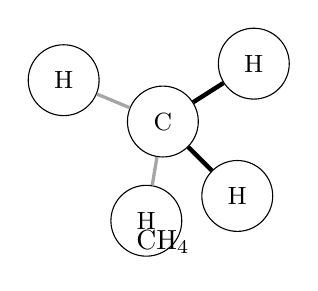
\begin{tikzpicture}[scale=1.05]
  \atom{C}{0}{0}{C}
  \atom{H1}{-1.2}{0.5}{H}
  \atom{H2}{1.1}{0.7}{H}
  \atom{H3}{-0.2}{-1.2}{H}
  \atom{H4}{0.9}{-0.9}{H}
  \bondback{C}{H1}
  \bondback{C}{H3}
  \bondfront{C}{H2}
  \bondfront{C}{H4}
  \node[below=8mm of C] {\(\ce{CH4}\)};
\end{tikzpicture}
\end{frame}

%------------------------------------------------
\begin{frame}{Aviation-specific: Jet A / Jet A-1 composition view}
\begin{itemize}
\item Broadly \(\mathrm{C_8\!-\!C_{16}}\), mixture of:
  \begin{itemize}
  \item iso-alkanes (cold-flow advantage)
  \item cyclo-alkanes (density contribution)
  \item aromatics (limited; seal swell vs soot)
  \end{itemize}
\item Combustor constraints: ignition, relight, LBO, soot (nvPM)
\end{itemize}
\end{frame}

%------------------------------------------------
\begin{frame}{Naming drill}
Name these:
\begin{enumerate}
\item \chemfig{H_3C-CH_2-CH_2-CH_2-CH_3}
\item \chemfig{H_3C-CH(-CH_3)-CH_2-CH_3}
\item \chemfig{H_3C-CH(-CH_3)-CH(-CH_3)-CH_3}
\item \chemfig{H_2C=CH-CH_2-CH_3}
\end{enumerate}

\vspace{2mm}

\end{frame}

%------------------------------------------------
\begin{frame}{Naming drill 2 (rings + aromatics)}

Name these:
\begin{enumerate}
\item \chemfig{*6(-=-=-(-CH_3)=)} 
\item \chemfig{*6(-(-CH_3)=(-CH_3)-=-=)} 
\end{enumerate}
\end{frame}

%------------------------------------------------
\begin{frame}{Naming drill 3 (lowest locants + alphabetical)}

Name this:

\chemfig{H_3C-CH(-CH_3)-CH_2-CH(-CH_2CH_3)-CH_3}

\end{frame}

%------------------------------------------------
\begin{frame}{Key Takeaways}

\begin{itemize}
\item Naming is a deterministic algorithm: parent \(\rightarrow\) numbering \(\rightarrow\) substituents
\item For fuels, naming immediately tells you: chain length, branching, ring/aromatic content
\item Structure \(\Rightarrow\) combustion: octane/cetane trends and soot propensity
\item Aviation adds cold-soak, stability, emissions constraints
\end{itemize}
\end{frame}

\end{document}
